% IE 643 course project, Stage 1 presentation (18 slides + references).
% Slide order follows "Instructions for Project Presentation Slides" in the intensive-assessment
% instructions. Numbers are the ones of record in report/IE643_Project_Report.tex.
%
% Build:  cd slides && latexmk -pdf IE643_Presentation.tex
% Figures: ../report/figures (copied from code/results/figures) and figures/ (make_slide_figures.py).

\documentclass[aspectratio=169,11pt]{beamer}
\usetheme{Madrid}
\setbeamertemplate{navigation symbols}{}
\setbeamertemplate{bibliography item}[text]
\setbeamerfont{frametitle}{size=\large}

\usepackage[utf8]{inputenc}
\usepackage{amsmath,amssymb,booktabs,tabularx,array}
\usepackage{tikz,pgfplots}
\usetikzlibrary{positioning,arrows.meta}
\pgfplotsset{compat=1.18}
\tikzset{box/.style={draw=black!60, rounded corners=2pt, align=center, font=\footnotesize,
                     minimum height=1.25cm, text width=2.25cm, fill=#1},
         box/.default=white}
\graphicspath{{figures/}{../report/figures/}}

\newcommand{\xs}{\bar{x}}
\newcommand{\xd}{\tilde{x}}
\newcommand{\dD}{\Delta D}
\newcommand{\code}[1]{\texttt{#1}}
\newcommand{\todo}[1]{\textcolor{red}{[#1]}}
\definecolor{motion}{HTML}{E8692F}
\definecolor{content}{HTML}{2A6FDB}

\title[Content vs.\ Motion in Video Diffusion U-Nets]
  {Probing the Latent Space of Video Diffusion U-Nets:\\Disentangling Content vs.\ Motion}
\subtitle{IE 643 (Deep Learning: Theory and Practice) Course Project, July--Dec 2026}
\author[Team Claudn't]{Team Claudn't\\[4pt]
  \small \todo{Member name 1} (\todo{roll number}) \quad \todo{Member name 2} (\todo{roll number})}
\institute[IIT Bombay]{Indian Institute of Technology Bombay}
\date[Stage 1, Oct 2026]{Intensive assessment, Stage 1 --- October 2026}

\begin{document}

% 1 --------------------------------------------------------------------------------------------
\begin{frame}
  \titlepage
\end{frame}

% 2 --------------------------------------------------------------------------------------------
\begin{frame}{Outline}
  \begin{columns}[T,onlytextwidth]
    \begin{column}{0.47\textwidth}
      \begin{enumerate}
        \item The task and what ``content'' and ``motion'' mean here
        \item Workflow: from the brief to a scored edit
        \item Before the prep review: model, hypotheses, pilots
        \item After the prep review
        \item Approach: model, probing, interventions, trained LoRAs
      \end{enumerate}
    \end{column}
    \begin{column}{0.47\textwidth}
      \begin{enumerate}\setcounter{enumi}{5}
        \item Data: 360 generated clips and 19 HMDB51 clips
        \item Experimental setup and the edit metric
        \item Results: where motion lives, edits, examples, LoRAs
        \item Conclusions
        \item Plan for novelty assessment
      \end{enumerate}
    \end{column}
  \end{columns}
\end{frame}

% 3 --------------------------------------------------------------------------------------------
\section{Problem}
\begin{frame}{The task: find where a video U-Net decides content and motion, then edit one alone}
  \begin{columns}[T,onlytextwidth]
    \begin{column}{0.5\textwidth}
      \textbf{Definitions (from the brief)}
      \begin{description}[Content]
        \item[\textcolor{content}{Content}] what one frame shows: identity, colour, texture, layout
        \item[\textcolor{motion}{Motion}] how pixels move across frames, whatever they belong to
      \end{description}
      \vspace{2mm}
      ``A golden retriever running on a beach'': the dog and the beach are content, the gait and
      path are motion. A disentangled model should let us keep the run and swap the dog for a
      horse, or keep the dog and make it walk.
    \end{column}
    \begin{column}{0.46\textwidth}
      \textbf{Deliverables}
      \begin{enumerate}\small
        \item Set up a small open video diffusion model; hook activations and attention
        \item Map which layers and timesteps carry content vs.\ motion
        \item An activation-patching framework that moves one between samples
        \item Edits in both directions, with a metric, an interface and a trained model
      \end{enumerate}
      \vspace{1mm}
      \begin{block}{Why it is not obvious}\small
        ``Spatial layers = content, temporal layers = motion'' is a statement about the wiring.
        Temporal layers write back into the same residual stream, and the verb reaches spatial
        layers through cross-attention.
      \end{block}
    \end{column}
  \end{columns}
\end{frame}

% 4 --------------------------------------------------------------------------------------------
\section{Workflow}
\begin{frame}{Workflow: each stage fixes what the next one is allowed to use}
  \centering
  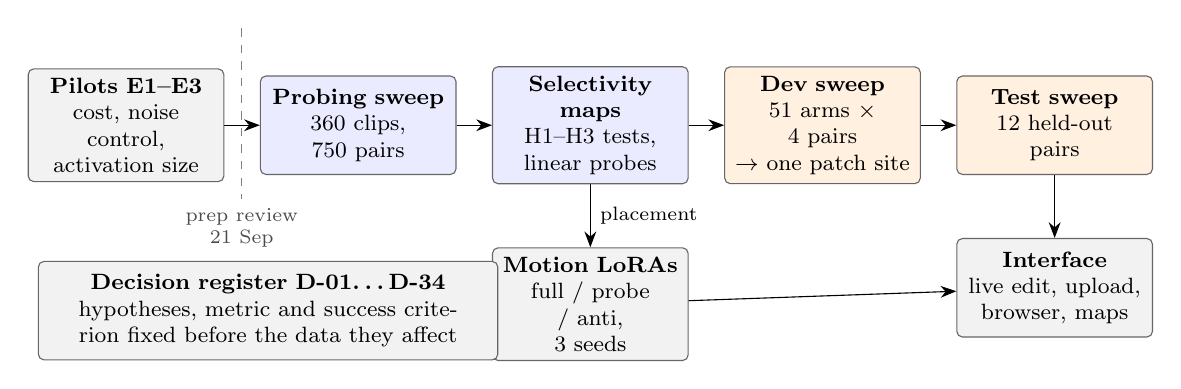
\begin{tikzpicture}[>={Stealth[length=2mm]}, node distance=0.45cm]
  \node[box=black!5] (p) {\textbf{Pilots E1--E3}\\cost, noise control,\\activation size};
  \node[box=blue!8, right=of p] (s) {\textbf{Probing sweep}\\360 clips,\\750 pairs};
  \node[box=blue!8, right=of s] (m) {\textbf{Selectivity maps}\\H1--H3 tests,\\linear probes};
  \node[box=orange!12, right=of m] (d) {\textbf{Dev sweep}\\51 arms $\times$ 4 pairs\\$\to$ one patch site};
  \node[box=orange!12, right=of d] (t) {\textbf{Test sweep}\\12 held-out\\pairs};
  \node[box=black!5, below=0.8cm of m] (l) {\textbf{Motion LoRAs}\\full / probe / anti,\\3 seeds};
  \node[box=black!5, below=0.8cm of t] (i) {\textbf{Interface}\\live edit, upload,\\browser, maps};
  \node[box=black!5, below=1.0cm of p, text width=5.6cm, anchor=north west, xshift=-1.12cm]
       (r) {\textbf{Decision register D-01\ldots D-34}\\hypotheses, metric and success
       criterion fixed before the data they affect};
  \draw[->] (p) -- (s); \draw[->] (s) -- (m); \draw[->] (m) -- (d); \draw[->] (d) -- (t);
  \draw[->] (m) -- node[right, font=\scriptsize]{placement} (l);
  \draw[->] (l) -- (i);
  \draw[->] (t) -- (i);
  \draw[dashed, black!50] ([xshift=-2.3mm,yshift=6mm]s.north west) -- ([xshift=-2.3mm,yshift=-3mm]s.south west)
     node[below, font=\scriptsize, black!70, align=center]{prep review\\21 Sep};
  \end{tikzpicture}

  \vspace{4mm}
  \small Left of the dashed line: September, before the prep review. Right: October. The maps
  choose where the dev sweep patches and where the map-guided LoRA sits; the dev sweep chooses
  the single configuration the test pairs are scored on.
\end{frame}

% 5 --------------------------------------------------------------------------------------------
\section{Before the prep review}
\begin{frame}{Before the review (1/2): AnimateDiff, and three hypotheses that could fail}
  \begin{columns}[T,onlytextwidth]
    \begin{column}{0.4\textwidth}
      \small
      \textbf{Model choice}\\[1mm]
      \begin{tabular}{@{}>{\raggedright}p{1.9cm}>{\raggedright\arraybackslash}p{3.9cm}@{}}
        \toprule
        AnimateDiff & explicit spatial/temporal split, fits a T4 (10.2\,GB) --- \textbf{chosen} \\
        \addlinespace ModelScope T2V & space and time trained jointly; thinner tooling --- kept for later \\
        \addlinespace Stable Video Diffusion & image-conditioned only, so no one-word prompt pairs \\
        \bottomrule
      \end{tabular}
    \end{column}
    \begin{column}{0.56\textwidth}
      \small
      \textbf{Hypotheses, each with a test fixed in advance}
      \begin{description}[H3]
        \item[H1] Motion selectivity peaks in a mid-resolution decoder block (\code{up\_blocks.1}),
          as MOFT \cite{xiao2024moft} suggests. \emph{Test:} bootstrap argmax over the 9 temporal
          blocks excludes the extreme resolutions.
        \item[H2] Motion is settled early in denoising. \emph{Test:} a least-squares changepoint
          $\tau$ falls in the first half.
        \item[H3] The frame mean $\xs$ is content; removing it reveals hidden motion. \emph{Test:}
          $\ge$75\% of cells content-selective in $\xs$, and some temporal cell flips sign in $\xd$.
      \end{description}
    \end{column}
  \end{columns}
\end{frame}

% 6 --------------------------------------------------------------------------------------------
\begin{frame}{Before the review (2/2): pilot E2 showed pixel motion is confounded by content}
  \begin{columns}[c,onlytextwidth]
    \begin{column}{0.55\textwidth}
      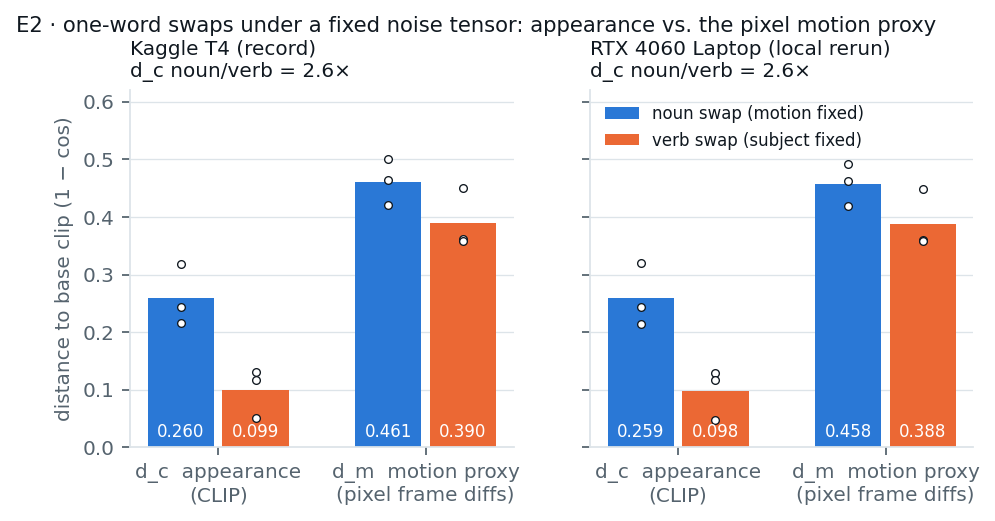
\includegraphics[width=\textwidth]{e2_pixel_confound.png}
    \end{column}
    \begin{column}{0.42\textwidth}
      \small
      \textbf{E2} Seven clips from one noise tensor. Subject swaps moved CLIP appearance
      2.6$\times$ more than verb swaps, but a frame-difference motion proxy moved \emph{more}
      under subject swaps (0.461) than verb swaps (0.390): a new animal has a new silhouette.

      $\Rightarrow$ measure motion inside the model, on the frame-varying part $\xd$, and swap
      subjects only within a body plan.

      \vspace{2mm}
      \textbf{E1} 94.1\,s and 10.2\,GB per clip on a T4: 360 clips $\approx$ 9.4 GPU-hours.

      \textbf{E3} Hooks on all 95 modules cost 0.6\%. A full dump is 87.9\,GiB per clip, so
      activations cannot be stored; pairs must be scored online.
    \end{column}
  \end{columns}
\end{frame}

% 7 --------------------------------------------------------------------------------------------
\section{After the prep review}
\begin{frame}{After the review: from pilots to a pre-registered test on held-out pairs}
  \small
  \begin{itemize}\setlength{\itemsep}{1.2mm}
    \item \textbf{Package \code{vdprobe}}: hooks, patching, a lockstep sampler that denoises 60 clips
      step by step; final latents identical to the diffusers pipeline (mean abs.\ diff.\ exactly 0).
    \item \textbf{Probing sweep} on Kaggle (2$\times$T4, 5.2\,h): 360 clips, 16 coordinates $\times$ 25
      steps, 300{,}000 distance rows; selectivity maps, H1--H3 tests, linear probes.
    \item \textbf{Component patching}, a new intervention built from the map's own split: move only
      $\xd$ or only $\xs$. Temporal-attention injection as the training-free baseline.
    \item \textbf{Controls on the real model} (null, mis-indexed, leakage, symmetry). They caught two
      fp16 bugs that the 51 unit tests missed.
    \item \textbf{Dev sweep} (51 arms, 4 pairs) picks one configuration per direction by a rule fixed
      before scoring; \textbf{test sweep} scores it on 12 frozen pairs.
    \item \textbf{Trained model}: motion LoRAs on HMDB51 placed by the map, everywhere, and in the wrong
      place; retrained on cut-free windows with 3 seeds after finding cuts in 11 of 19 clips.
    \item \textbf{Gradio interface}: live edits, uploaded videos, a browser of every scored clip, the maps.
  \end{itemize}
\end{frame}

% 8 --------------------------------------------------------------------------------------------
\section{Approach}
\begin{frame}{Approach (1/3): AnimateDiff adds 21 temporal modules to a frozen image U-Net}
  \centering
  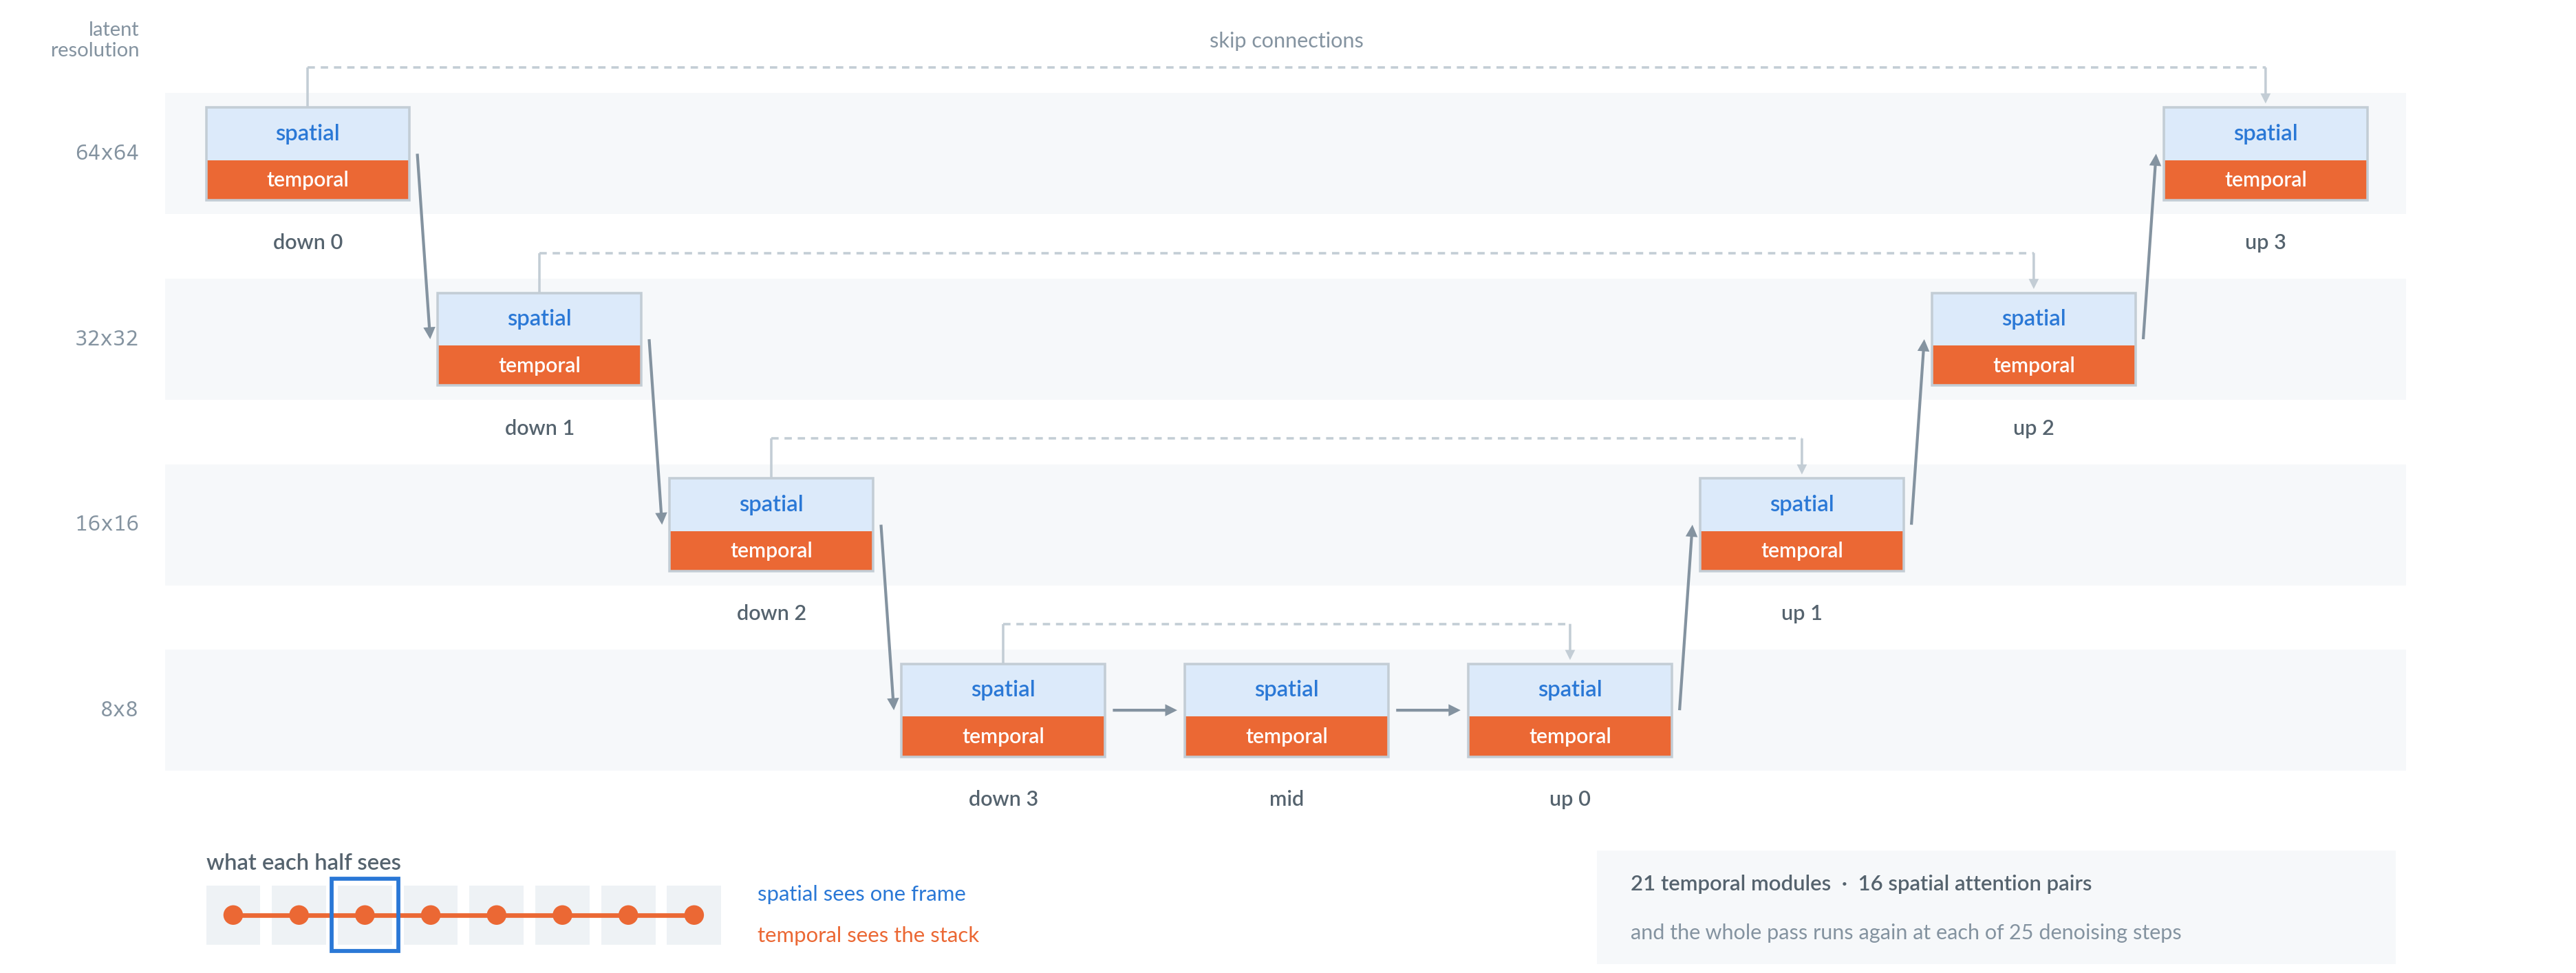
\includegraphics[height=4.1cm]{unet.png}

  \vspace{2mm}
  \begin{columns}[T,onlytextwidth]
    \begin{column}{0.5\textwidth}
      \footnotesize
      SD-1.5 U-Net (860\,M, frozen) + motion adapter v1-5-2 (417\,M). Spatial transformers see one
      frame and cross-attend to the CLIP text; each motion module attends over the 16 frames at one
      position and adds the result back. 25 DDIM steps, CFG 7.5, 512$^2$, 16 frames.
    \end{column}
    \begin{column}{0.46\textwidth}
      \footnotesize
      Every activation $x\in\mathbb{R}^{F\times C\times S}$ is split into
      \[
        \underbrace{\xs = \tfrac{1}{F}\textstyle\sum_f x_f}_{\text{static}}, \qquad \underbrace{\xd = x-\xs}_{\text{frame-varying}}
      \]
      Distance between two clips at a coordinate: $d = 1-\cos(a,b)$, on $\xs$ and $\xd$ separately.
    \end{column}
  \end{columns}
\end{frame}

% 9 --------------------------------------------------------------------------------------------
\begin{frame}{Approach (2/3): selectivity weighs a subject swap against a verb swap}
  \begin{columns}[T,onlytextwidth]
    \begin{column}{0.5\textwidth}
      \small
      \textbf{Selectivity} at layer $L$, step $t$:
      \[
        S = \frac{d_c - d_m}{d_c + d_m}\in[-1,1]
      \]
      $d_c$: subject swapped, $d_m$: verb swapped. $S>0$ = \textcolor{content}{content-selective},
      $S<0$ = \textcolor{motion}{motion-selective}. $S_{dyn}$ on $\xd$, $S_{stat}$ on $\xs$.

      Matched units: clip B is the end point of one content pair and one motion pair, 78 units
      per seed; median over units, 1{,}000-sample bootstrap CI, averaged over 3 seeds.

      \textbf{Linear probes} for verb (4 classes) and family (2) on count-sketched $\xd,\xs$
      (512-d), trained on one scene and tested on the other.
    \end{column}
    \begin{column}{0.46\textwidth}
      \small
      \textbf{Lockstep sampler}\\
      Caching an anchor's activations for 25 steps takes 7.6\,GB. Instead, all 60 clips of a
      (seed, scene) group are denoised together:
      \begin{enumerate}
        \item step $t$: run every anchor, keep its step-$t$ activations
        \item run every partner, score it against them on the full tensors
        \item drop step $t$; continue
      \end{enumerate}
      Memory holds one step instead of 25, and every clip is generated exactly once.
    \end{column}
  \end{columns}
\end{frame}

% 10 -------------------------------------------------------------------------------------------
\begin{frame}{Approach (3/3): two ways to transplant motion, and one trained model}
  \begin{columns}[T,onlytextwidth]
    \begin{column}{0.31\textwidth}
      \footnotesize
      \textbf{Component patch} (ours)\\
      dynamic: $x \leftarrow \xs_{tgt} + \xd_{src}$\\
      static:\phantom{y} $x \leftarrow \xs_{src} + \xd_{tgt}$

      \vspace{1mm}
      Computed as $x + (\delta - \bar\delta)$ with $\delta = x_{src}-x$, so a self-patch is
      exactly zero in fp16. A whole-tensor patch on a motion module copies content too; the split
      is meant to move one and keep the other.
    \end{column}
    \begin{column}{0.31\textwidth}
      \footnotesize
      \textbf{Attention injection} (baseline)\\
      The target uses the source's temporal attention probabilities $P_{src}$ with its own $V$:
      \[
        \begin{aligned}&\mathrm{SDPA}(Q,K,V)\\ &+ \alpha\,W_{out}\big((P_{src}-P)V\big)\end{aligned}
      \]
      MotionClone's \cite{ling2025motionclone} idea without gradient guidance.
    \end{column}
    \begin{column}{0.33\textwidth}
      \footnotesize
      \textbf{Motion LoRA} \cite{hu2022lora} on Q, K, V, O of temporal attention, rank 32:
      \begin{itemize}
        \item \code{full}: all 21 modules, 9.67\,M
        \item \code{probe}: \code{up\_blocks.0} (map peak), 1.97\,M
        \item \code{anti}: \code{down\_blocks.2,3} (map minimum), 2.62\,M
      \end{itemize}
      \[
        \mathcal{L} = \mathbb{E}\,\big\|\epsilon - \epsilon_\theta(z_t, t, c)\big\|_2^2
      \]
      on VAE latents of real clips; only LoRA weights train.
    \end{column}
  \end{columns}
\end{frame}

% 11 -------------------------------------------------------------------------------------------
\section{Data}
\begin{frame}{Data: the model generates its own probing set; HMDB51 trains the LoRAs}
  \begin{columns}[T,onlytextwidth]
    \begin{column}{0.53\textwidth}
      \small
      \textbf{Generated probing set} --- ``a \{subject\} \{verb\} \{scene\}, high quality, detailed''
      \begin{itemize}
        \item 15 subjects in 2 body-plan families (8 quadrupeds, 7 humans), 4 verbs (running,
          walking, jumping, spinning), 2 scenes, 3 seeds
        \item 120 clips per seed, \textbf{360 clips}, 16 frames of 512$\times$512
        \item one noise tensor per (seed, scene) group, so a pair differs only by its word
        \item per seed: 104 content pairs, 90 motion pairs, 56 cross-family pairs; \textbf{750 pairs}
      \end{itemize}
      \textbf{Edit pairs}: 12 test + 4 dev, A and B differ in subject \emph{and} verb; frozen before
      any edit ran.
    \end{column}
    \begin{column}{0.43\textwidth}
      \small
      \textbf{HMDB51} \cite{kuehne2011hmdb} (HF mirror \code{divm/hmdb51}, pinned)
      \begin{itemize}
        \item classes run, walk, jump, turn
        \item filter on HMDB tags: full body, no camera motion, one person, quality not bad,
          one clip per film $\to$ \textbf{19 clips}, 2.0\,MB
        \item 15 train / 4 validation (last clip of each class)
      \end{itemize}
      \textbf{Preprocessing}: 16 frames at stride $\le 2$, random full-height square crop, resize to
      256$^2$, scale to $[-1,1]$, frozen VAE. \textbf{Cut-free} recipe: 11 clips contain a scene
      cut, so each window is drawn inside one shot.
    \end{column}
  \end{columns}
\end{frame}

% 12 -------------------------------------------------------------------------------------------
\section{Experiments}
\begin{frame}{Setup: one metric $D$ rewards taking the right property from each clip}
  \begin{columns}[T,onlytextwidth]
    \begin{column}{0.45\textwidth}
      \small
      \textbf{Hardware}: laptop RTX 4060 8\,GB (development, controls, scoring, interface);
      Kaggle 2$\times$T4 16\,GB (sweeps, cut-free LoRAs). 65\,s per clip on the laptop, 90--97\,s on a T4.

      \textbf{Software}: PyTorch 2.10, diffusers 0.40, PEFT 0.21.2, scikit-learn, OpenCV, Gradio 6.

      \textbf{LoRA training}: AdamW, lr $5\times10^{-5}$, weight decay $10^{-2}$, batch 1, 800 steps,
      $t\sim U\{1..1000\}$, fp16 base with fp32 LoRA, checkpointed motion modules (5.0\,GB peak).

      \textbf{Code}: \url{https://github.com/rujulaaaa/IE643}
    \end{column}
    \begin{column}{0.51\textwidth}
      \footnotesize
      \textbf{Motion direction}: output should look like B and move like A.
      \[
        \begin{aligned}
        D = {}&\tfrac12\big[\hat s_c(\text{out},B) + \hat s_m(\text{out},A)\big] && \text{right property}\\
          -{}&\tfrac12\big[\hat s_c(\text{out},A) + \hat s_m(\text{out},B)\big] && \text{wrong property}
        \end{aligned}
      \]
      $s_c$: per-frame CLIP image cosine; $s_m$: cosine of Farneb\"ack optical flow;
      $\hat s$ min-max normalised per run. Content direction swaps A and B.

      \textbf{Reported}: $\dD = D(\text{arm}) - D(\text{prompt only})$ on the same pair.

      \begin{block}{Success criterion (D-16, fixed in advance)}\footnotesize
        In both directions: median $\dD>0$, its 95\% paired-bootstrap CI excludes 0, and subject
        consistency within 10\% of the source.
      \end{block}
    \end{column}
  \end{columns}
\end{frame}

% 13 -------------------------------------------------------------------------------------------
\section{Results}
\begin{frame}{Content dominates almost every layer; motion wins in one block, for 2--3 steps}
  \centering
  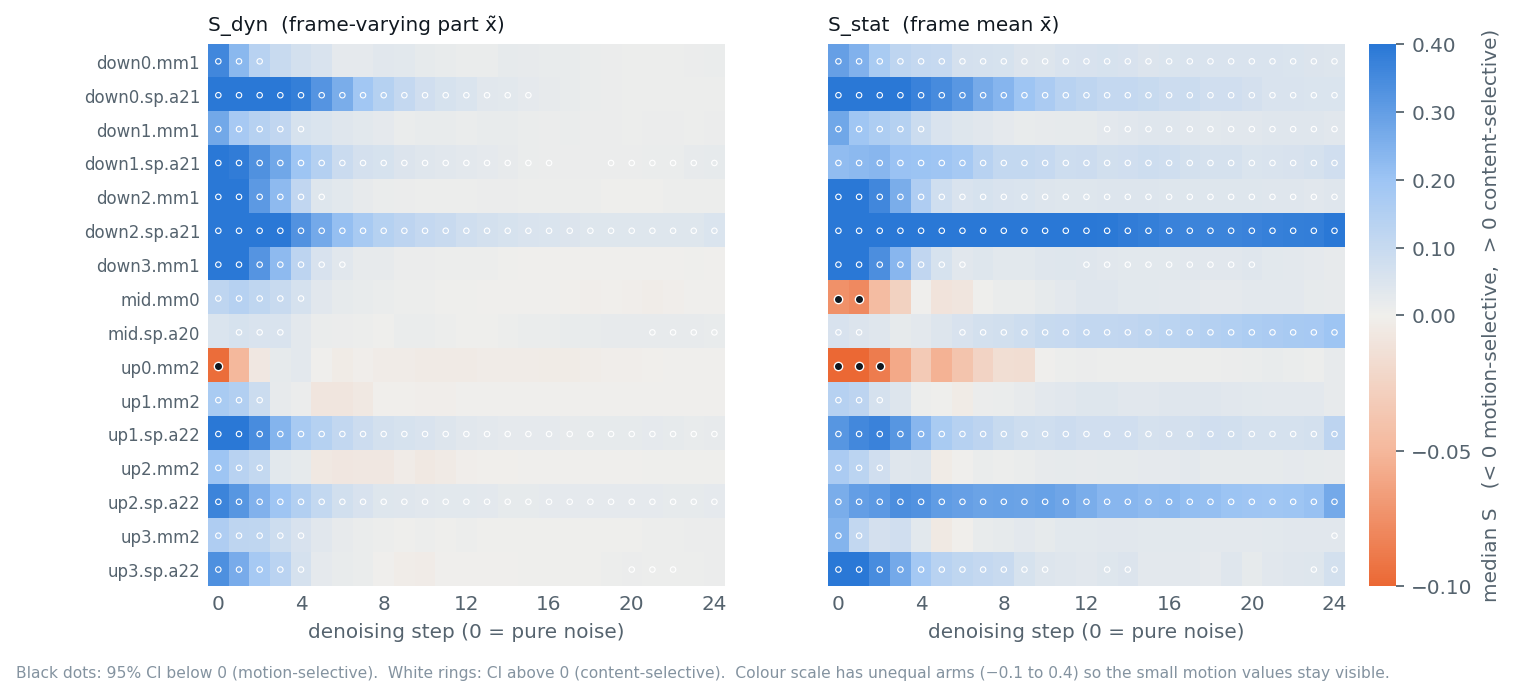
\includegraphics[height=5.0cm]{sweep_selectivity_maps.png}

  \vspace{1mm}
  \footnotesize
  \setlength{\tabcolsep}{4pt}\begin{tabularx}{\textwidth}{@{}lp{1.4cm}X@{}}
    \toprule
    H1 layer & \textcolor{red!70!black}{falsified} & peak at \code{up\_blocks.0} (8$\times$8) in 1000/1000 resamples; every other block $<0$ \\
    H2 timestep & \textcolor{green!45!black}{survives} & changepoint $\tau = 2$, 95\% CI [1, 3]; early mean 0.073 vs.\ late $-$0.001 \\
    H3 representation & \textcolor{red!70!black}{falsified} & 65\% $<$ 75\% content-selective in $\xs$; no cell flips; early motion is cleaner in $\xs$ \\
    \bottomrule
  \end{tabularx}
\end{frame}

% 14 -------------------------------------------------------------------------------------------
\begin{frame}{On 12 held-out pairs, only attention injection clearly beats changing the prompt}
  \begin{columns}[c,onlytextwidth]
    \begin{column}{0.6\textwidth}
      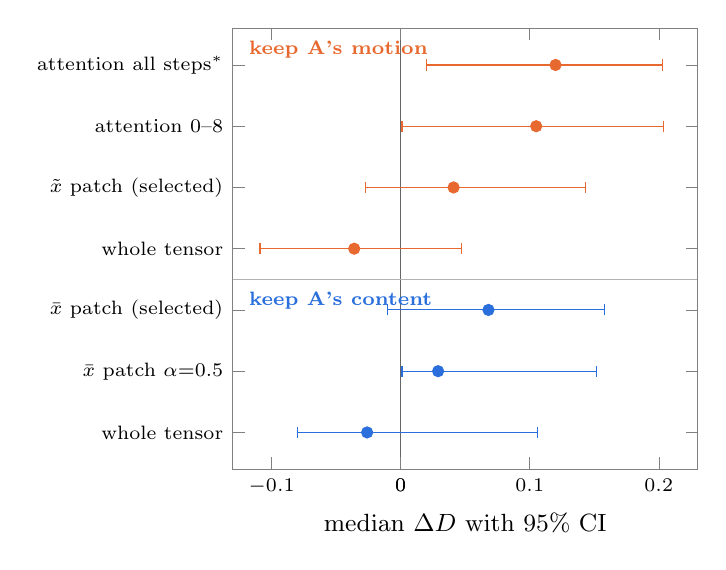
\begin{tikzpicture}
      \begin{axis}[
        scale only axis, width=5.9cm, height=5.6cm, xmin=-0.13, xmax=0.23,
        ytick={1,...,7}, yticklabel style={font=\scriptsize, align=right},
        yticklabels={whole tensor, $\xs$ patch $\alpha$=0.5, $\xs$ patch (selected),
                     whole tensor, $\xd$ patch (selected), attention 0--8, attention all steps$^*$},
        xlabel={median $\dD$ with 95\% CI}, xlabel style={font=\small},
        xticklabel style={font=\scriptsize, /pgf/number format/fixed},
        extra x ticks={0}, extra x tick style={grid=major, grid style={black!60}},
        ymin=0.4, ymax=7.6, enlarge y limits=false, axis line style={black!50},
        tick style={black!50}]
        \addplot[only marks, mark=*, content, error bars/.cd, x dir=both, x explicit] coordinates {
          (-0.026,1) -= (0.054,0) += (0.132,0)
          (0.029,2)  -= (0.028,0) += (0.123,0)
          (0.068,3)  -= (0.078,0) += (0.090,0)};
        \addplot[only marks, mark=*, motion, error bars/.cd, x dir=both, x explicit] coordinates {
          (-0.036,4) -= (0.073,0) += (0.083,0)
          (0.041,5)  -= (0.068,0) += (0.102,0)
          (0.105,6)  -= (0.104,0) += (0.099,0)
          (0.120,7)  -= (0.100,0) += (0.083,0)};
        \draw[black!30] (axis cs:-0.13,3.5) -- (axis cs:0.23,3.5);
        \node[font=\scriptsize\bfseries, motion, anchor=north west] at (axis cs:-0.125,7.55) {keep A's motion};
        \node[font=\scriptsize\bfseries, content, anchor=north west] at (axis cs:-0.125,3.45) {keep A's content};
      \end{axis}
      \end{tikzpicture}
    \end{column}
    \begin{column}{0.37\textwidth}
      \footnotesize
      \begin{itemize}\setlength{\itemsep}{1mm}
        \item The pre-registered criterion is \textbf{not met}: the selected component patches are
          positive on 8/12 and 10/12 pairs, but their CIs include 0.
        \item Component patches beat whole-tensor patches at the same site in both directions;
          the whole tensor drags A's look along ($s_c(\text{out},A)=0.91$).
        \item Attention injection over all 25 steps: +0.120, 11/12 pairs, CI [0.020, 0.203].
        \item The best patch site is \code{up\_blocks.3}, not the map's peak \code{up\_blocks.0} (+0.030).
      \end{itemize}
      \scriptsize $^*$scored in one pool with the LoRA run (bit-identical regenerated clips).
    \end{column}
  \end{columns}
\end{frame}

% 15 -------------------------------------------------------------------------------------------
\begin{frame}{Test pair 1: the patched horse picks up the dog's splash and stride}
  \centering
  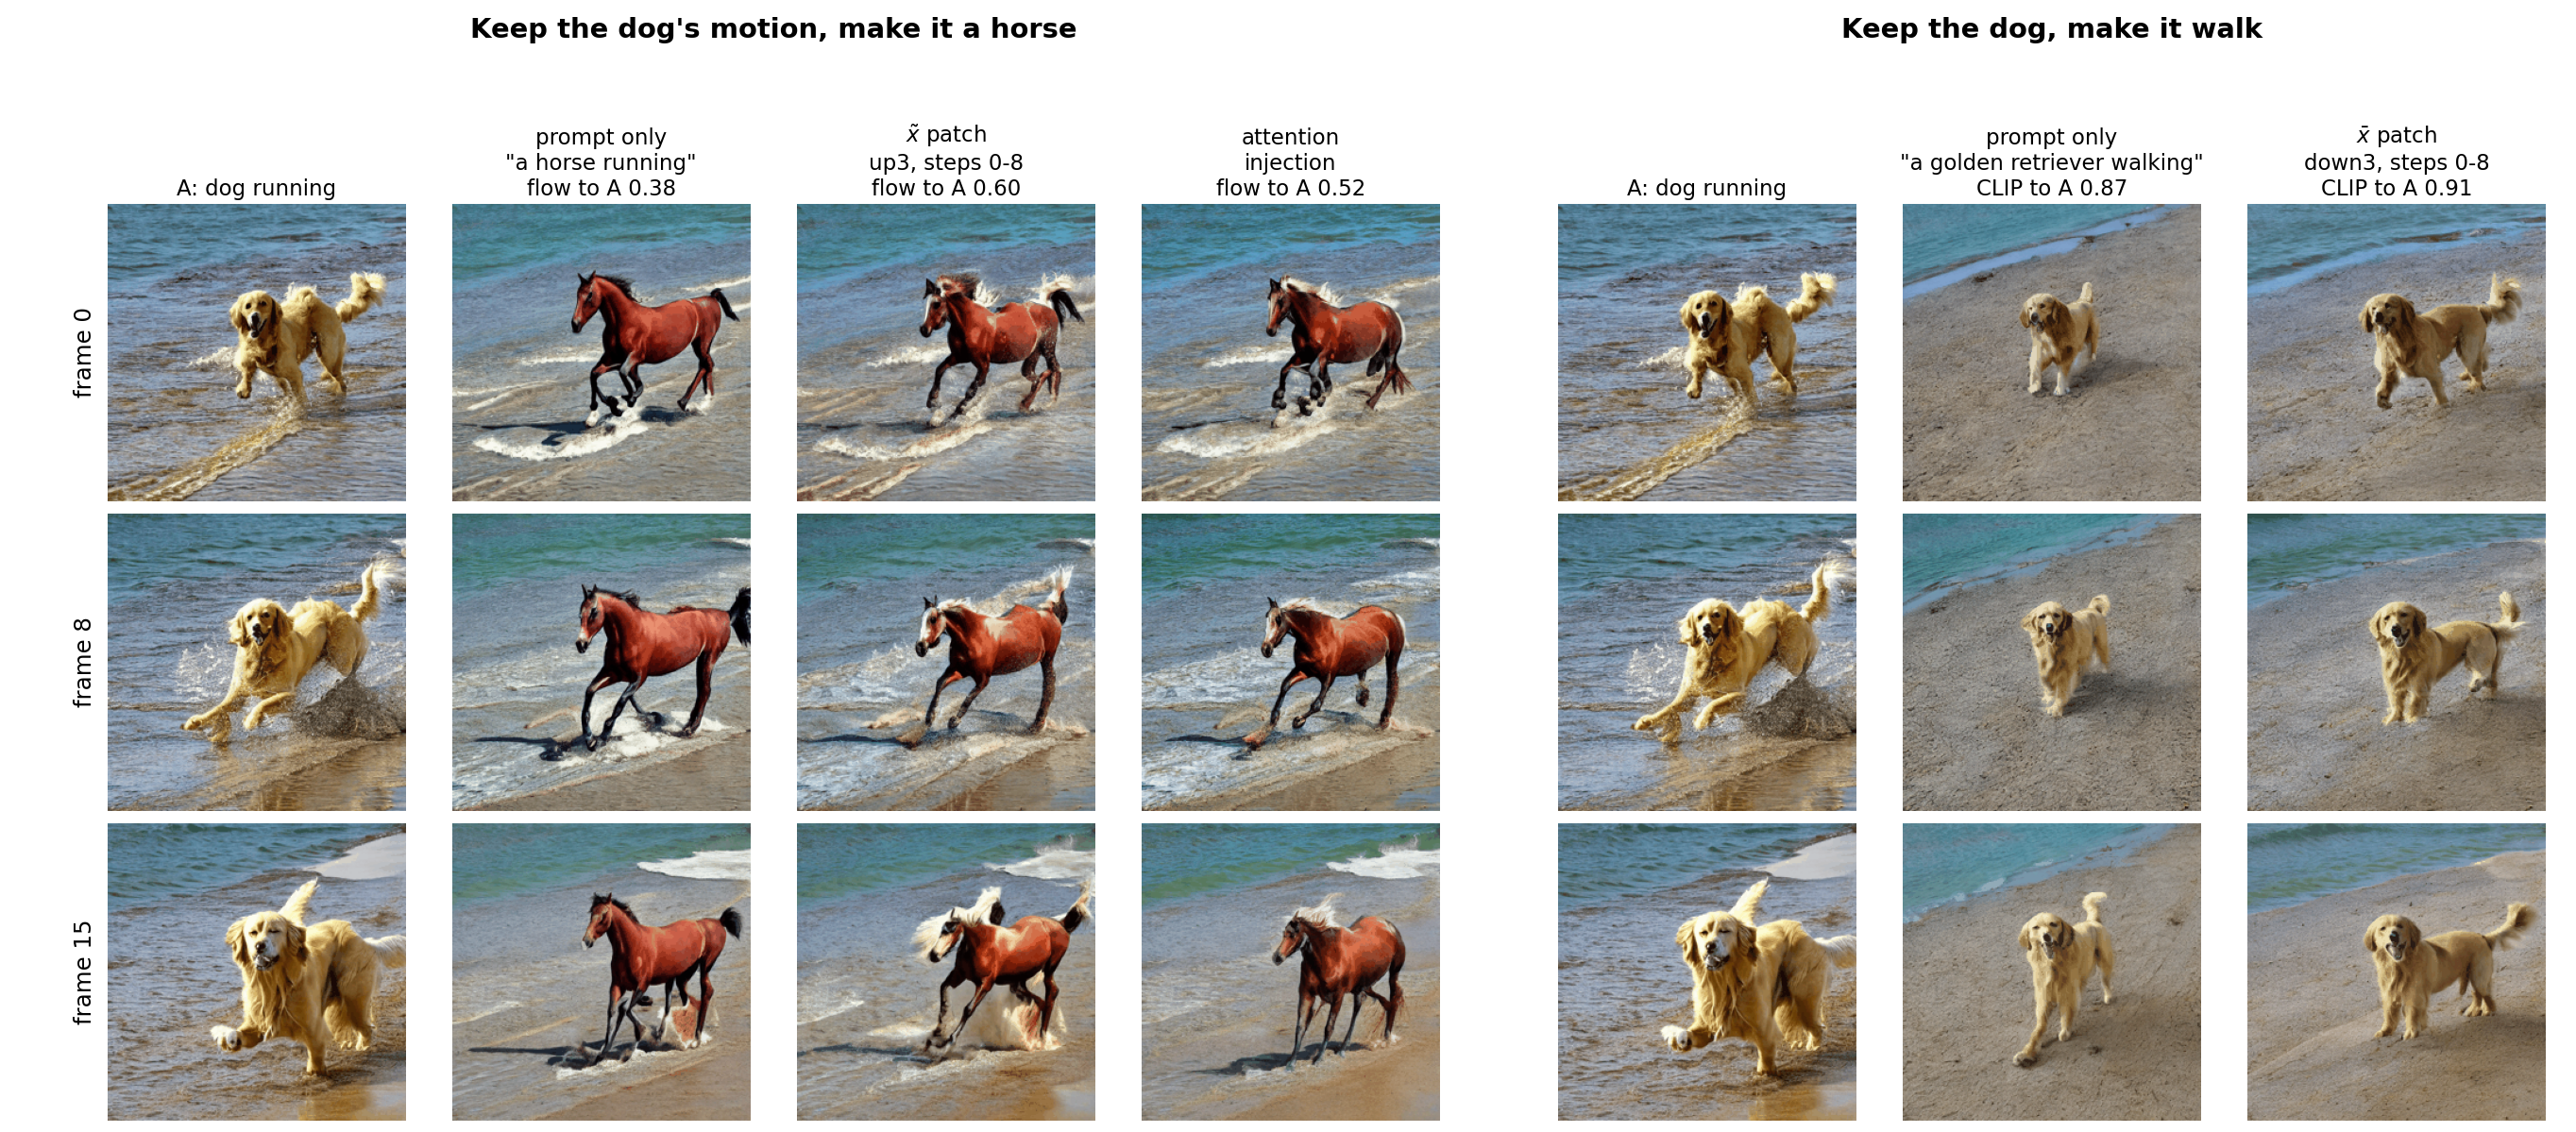
\includegraphics[height=6.0cm]{qual_wide_42.png}

  \vspace{1mm}
  \footnotesize Beach, seed 42; B is ``a horse walking''. The $\xd$ patch brings A's motion (flow 0.38 $\to$ 0.60)
  and some of A's look (pale mane, spray). The $\xs$ patch keeps the dog's build and raised tail as it walks.
\end{frame}

% 16 -------------------------------------------------------------------------------------------
\begin{frame}{The trained model: the map-guided LoRA is the only one positive in all three seeds}
  \begin{columns}[c,onlytextwidth]
    \begin{column}{0.57\textwidth}
      \scriptsize\setlength{\tabcolsep}{4pt}
      \begin{tabular}{@{}lrcc@{}}
        \toprule
        LoRA & params & held-out loss & median $\dD$, seeds 0/1/2 \\
        \midrule
        untrained & -- & 0.0982 & -- \\
        \code{full}  & 9.67\,M & \textbf{0.0627} & +0.004 / +0.008 / $-$0.013 \\
        \code{probe} & 1.97\,M & 0.0641 & \textbf{+0.014 / +0.015 / +0.009} \\
        \code{anti}  & 2.62\,M & 0.0635 & $-$0.011 / $-$0.031 / $-$0.001 \\
        \bottomrule
      \end{tabular}

      \vspace{2mm}
      \footnotesize
      \begin{itemize}
        \item On loss, size beats placement: \code{anti} ends below \code{probe}; seed spread $<10^{-4}$.
        \item On the edit, \code{probe} is ahead, but by a small margin and no CI excludes 0.
        \item The gain comes from moving \emph{less like B} ($s_m$ 0.17 $\to$ 0.06--0.08), not more
          like A: the LoRA learned generic HMDB51 motion, not clip A's.
      \end{itemize}
    \end{column}
    \begin{column}{0.39\textwidth}
      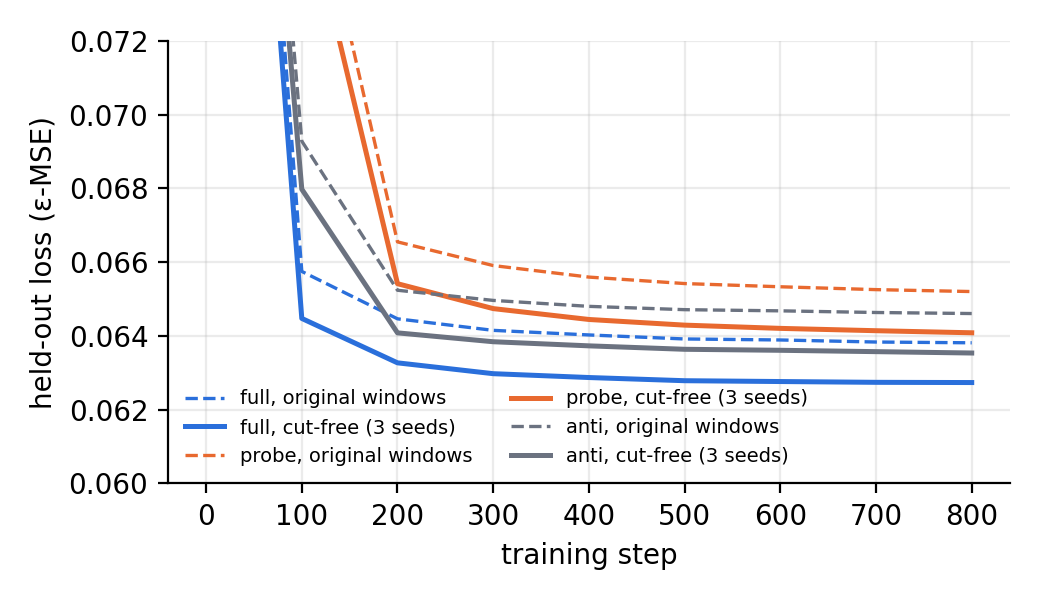
\includegraphics[width=\textwidth]{lora_val.png}

      \footnotesize Most of the loss drop is in the first 100 steps, which looks like adapting to
      HMDB51's grain and resolution more than to its motion.
    \end{column}
  \end{columns}
\end{frame}

% 17 -------------------------------------------------------------------------------------------
\section{Conclusions}
\begin{frame}{Conclusions}
  \begin{columns}[T,onlytextwidth]
    \begin{column}{0.48\textwidth}
      \small
      \textbf{What we found}
      \begin{itemize}\setlength{\itemsep}{1mm}
        \item The spatial/temporal wiring overstates the separation: content dominates nearly every
          layer, temporal ones included.
        \item Motion is selective only in the motion module after the bottleneck, during the first
          2--3 of 25 steps. H1 and H3 falsified, H2 survives.
        \item Where motion is \emph{represented} is not where patching \emph{uses} it best.
      \end{itemize}
    \end{column}
    \begin{column}{0.48\textwidth}
      \small
      \textbf{What it means for editing}
      \begin{itemize}\setlength{\itemsep}{1mm}
        \item Component patches beat the prompt and whole-tensor patching in both directions, but
          12 pairs cannot confirm it.
        \item Attention injection over all steps is the one edit clearly above zero (+0.120).
        \item For uploads only attention injection survives (flow to upload 0.66 vs.\ 0.03 for the
          patch); it moves \emph{where} things move, not \emph{which} object.
        \item Null patches are bit-exact and every rule was fixed in advance, so the negative
          results stand as results.
      \end{itemize}
    \end{column}
  \end{columns}
\end{frame}

% 18 -------------------------------------------------------------------------------------------
\section{Plan for novelty assessment}
\begin{frame}{Plan for novelty assessment: four open questions, four experiments}
  \small
  \begin{tabularx}{\textwidth}{@{}p{4.3cm}Xp{3.3cm}@{}}
    \toprule
    Open question & Experiment & Decided by \\
    \midrule
    Is the map an artefact of AnimateDiff's frozen backbone? &
      Same sweep, vocabulary and H1--H3 tests on a jointly trained model (ModelScope T2V or VideoCrafter2) &
      whether H1--H3 verdicts repeat \\[1mm]
    Can motion land on the right object? &
      Attention injection masked by the subject's cross-attention; same 12 pairs and the upload path &
      $\dD$ vs.\ unmasked injection \\[1mm]
    Are the near-misses real? &
      24 new pairs drawn by the same rule; symmetry control on all pairs, not one &
      CIs on 36 pairs \\[1mm]
    Are the metrics measuring motion? &
      CoTracker \cite{karaev2024cotracker} point tracks instead of flow cosine; DINO instead of CLIP;
      LoRA update ranking normalised per resolution &
      agreement with current rankings \\
    \bottomrule
  \end{tabularx}
\end{frame}

% References (not counted) ---------------------------------------------------------------------
\section*{References}
\begin{frame}{References (1/2)}
  \tiny\vspace*{-3mm}
  \begin{thebibliography}{99}\setlength{\itemsep}{0pt}
  \bibitem{guo2024animatediff} Yuwei Guo, Ceyuan Yang, Anyi Rao, Zhengyang Liang, Yaohui Wang, Yu Qiao, Maneesh Agrawala, Dahua Lin, and Bo Dai. AnimateDiff: Animate your personalized text-to-image diffusion models without specific tuning, ICLR, 2024. \url{https://arxiv.org/abs/2307.04725}
  \bibitem{xiao2024moft} Zeqi Xiao, Yifan Zhou, Shuai Yang, and Xingang Pan. Video diffusion models are training-free motion interpreter and controller, NeurIPS, 2024. \url{https://arxiv.org/abs/2405.14864}
  \bibitem{ling2025motionclone} Pengyang Ling, Jiazi Bu, Pan Zhang, Xiaoyi Dong, Yuhang Zang, Tong Wu, Huaian Chen, Jiaqi Wang, and Yi Jin. MotionClone: Training-free motion cloning for controllable video generation, ICLR, 2025. \url{https://arxiv.org/abs/2406.05338}
  \bibitem{meng2022rome} Kevin Meng, David Bau, Alex Andonian, and Yonatan Belinkov. Locating and editing factual associations in GPT, NeurIPS, 2022. \url{https://arxiv.org/abs/2202.05262}
  \bibitem{wang2023ioi} Kevin Wang, Alexandre Variengien, Arthur Conmy, Buck Shlegeris, and Jacob Steinhardt. Interpretability in the wild: A circuit for indirect object identification in GPT-2 small, ICLR, 2023. \url{https://arxiv.org/abs/2211.00593}
  \bibitem{zhang2024patching} Fred Zhang and Neel Nanda. Towards best practices of activation patching in language models: Metrics and methods, ICLR, 2024. \url{https://arxiv.org/abs/2309.16042}
  \bibitem{ho2022vdm} Jonathan Ho, Tim Salimans, Alexey Gritsenko, William Chan, Mohammad Norouzi, and David J. Fleet. Video diffusion models, NeurIPS, 2022. \url{https://arxiv.org/abs/2204.03458}
  \bibitem{blattmann2023align} Andreas Blattmann, Robin Rombach, Huan Ling, Tim Dockhorn, Seung Wook Kim, Sanja Fidler, and Karsten Kreis. Align your latents: High-resolution video synthesis with latent diffusion models, CVPR, 2023. \url{https://arxiv.org/abs/2304.08818}
  \bibitem{rombach2022ldm} Robin Rombach, Andreas Blattmann, Dominik Lorenz, Patrick Esser, and Bj\"orn Ommer. High-resolution image synthesis with latent diffusion models, CVPR, 2022. \url{https://arxiv.org/abs/2112.10752}
  \bibitem{song2021ddim} Jiaming Song, Chenlin Meng, and Stefano Ermon. Denoising diffusion implicit models, ICLR, 2021. \url{https://arxiv.org/abs/2010.02502}
  \bibitem{yatim2024dmt} Danah Yatim, Rafail Fridman, Omer Bar-Tal, Yoni Kasten, and Tali Dekel. Space-time diffusion features for zero-shot text-driven motion transfer, CVPR, 2024. \url{https://arxiv.org/abs/2311.17009}
  \bibitem{wu2023tav} Jay Zhangjie Wu, Yixiao Ge, Xintao Wang, Stan Weixian Lei, Yuchao Gu, Yufei Shi, Wynne Hsu, Ying Shan, Xiaohu Qie, and Mike Zheng Shou. Tune-A-Video: One-shot tuning of image diffusion models for text-to-video generation, ICCV, 2023. \url{https://arxiv.org/abs/2212.11565}
  \end{thebibliography}
\end{frame}

\begin{frame}{References (2/2)}
  \tiny
  \begin{thebibliography}{99}\setlength{\itemsep}{0pt}\setcounter{enumiv}{12}
  \bibitem{zhao2024motiondirector} Rui Zhao, Yuchao Gu, Jay Zhangjie Wu, David Junhao Zhang, Jiawei Liu, Weijia Wu, Jussi Keppo, and Mike Zheng Shou. MotionDirector: Motion customization of text-to-video diffusion models, ECCV, 2024. \url{https://arxiv.org/abs/2310.08465}
  \bibitem{hu2022lora} Edward J. Hu, Yelong Shen, Phillip Wallis, Zeyuan Allen-Zhu, Yuanzhi Li, Shean Wang, Lu Wang, and Weizhu Chen. LoRA: Low-rank adaptation of large language models, ICLR, 2022. \url{https://arxiv.org/abs/2106.09685}
  \bibitem{hertz2023p2p} Amir Hertz, Ron Mokady, Jay Tenenbaum, Kfir Aberman, Yael Pritch, and Daniel Cohen-Or. Prompt-to-prompt image editing with cross attention control, ICLR, 2023. \url{https://arxiv.org/abs/2208.01626}
  \bibitem{tang2023daam} Raphael Tang, Linqing Liu, Akshat Pandey, Zhiying Jiang, Gefei Yang, Karun Kumar, Pontus Stenetorp, Jimmy Lin, and Ferhan Ture. What the DAAM: Interpreting Stable Diffusion using cross attention, ACL, 2023. \url{https://arxiv.org/abs/2210.04885}
  \bibitem{baherwani2025timesteps} Vatsal Baherwani, Yixuan Ren, and Abhinav Shrivastava. Characterizing motion encoding in video diffusion timesteps, arXiv preprint, 2025. \url{https://arxiv.org/abs/2512.22175}
  \bibitem{radford2021clip} Alec Radford, Jong Wook Kim, Chris Hallacy, Aditya Ramesh, Gabriel Goh, Sandhini Agarwal, Girish Sastry, Amanda Askell, Pamela Mishkin, Jack Clark, Gretchen Krueger, and Ilya Sutskever. Learning transferable visual models from natural language supervision, ICML, 2021. \url{https://arxiv.org/abs/2103.00020}
  \bibitem{farneback2003} Gunnar Farneb\"ack. Two-frame motion estimation based on polynomial expansion, SCIA, 2003. \url{https://doi.org/10.1007/3-540-45103-X_50}
  \bibitem{kuehne2011hmdb} Hildegard Kuehne, Hueihan Jhuang, Est\'ibaliz Garrote, Tomaso Poggio, and Thomas Serre. HMDB: A large video database for human motion recognition, ICCV, 2011. \url{https://doi.org/10.1109/ICCV.2011.6126543}
  \bibitem{karaev2024cotracker} Nikita Karaev, Ignacio Rocco, Benjamin Graham, Natalia Neverova, Andrea Vedaldi, and Christian Rupprecht. CoTracker: It is better to track together, ECCV, 2024. \url{https://arxiv.org/abs/2307.07635}
  \bibitem{hf_animatediff} Yuwei Guo and others. \url{https://huggingface.co/guoyww/animatediff-motion-adapter-v1-5-2}, Accessed on: 20th October, 2026.
  \bibitem{hf_diffusers} Hugging Face. \url{https://huggingface.co/docs/diffusers}, Accessed on: 20th October, 2026.
  \bibitem{hf_hmdb} DIVM. \url{https://huggingface.co/datasets/divm/hmdb51}, Accessed on: 20th October, 2026.
  \end{thebibliography}
\end{frame}

\end{document}
